\chapter{Part J: Convertible Bonds}
Developer: Aloke Mukherjee

\noindent Validator: Jospeh Perez


%DEVELOPER WRITES THIS PART --->

\section{Requirements}

%<description of the problem being solved, relevant equations, algorithms, etc>
A convertible bond behaves as a hybrid between a bond and a stock
because in addition to the principal guarantee and coupons it can
also be converted into a specified number of shares of stock at
given times.  As the chance of converting increases due to stock
price appreciation the price of convertible bonds will behave more
like the stock.  If the chance of converting is low then the
convertible's price will be more affected by interest rates and its
behaviour is more bond-like.

This "early-exercise" feature of convertible bonds makes it
difficult to model with Monte Carlo simulation.  Instead a binomial
tree is used to model the underlying stock price.  The convertible
bond is then evaluated at leaf nodes as the maximum of the par value
and the conversion value and these values are propagated back to the
tree's root.

An additional complication is the callability and putability
features of convertible bonds.  Callability allows the issuer to
call back the bond at a set price.  Putability conversely allows the
owner the put the bond back to the issuer at a set price.  This
optionality can also be modelled in the binomial tree by evaluating
at each step whether it is optimal for either party to exercise
their option.

\section{Design }

We constructed a binomial tree class which can store the
intermediate stock process and claim process values.  At
instantiation this class uses the yield curve and the stock's price
and volatility to calculate and cache the magnitude of each up and
down jump. The Cox-Ross-Rubinstein values are used - namely up moves
are $e^{\sigma\surd t}$ and down moves are the reciprocal of this.
The probability of an up move is the difference between the riskfree
value at the next node and the down value divided by the difference
between the up and down values.  The probability of a down move is
the complement.  We use the yield curve's ability to compute forward
discount factors to compute discount factors and probabilities for
each step of the tree.  If a flat yield curve is specified these
will all be the same but the design allows the use of a more
realistic yield curve.

Evaluation of the claim process is based on the same technique used
in the Monte Carlo simulation: different "Engine" methods are
defined in the binomial tree class which can be used to evaluate
different claim processes. The engine uses a standard PayOff object
used throughout the project to evaluate the claim at terminal nodes.
The engine applies risk-neutral probabilities to discount the payoff
as well as evaluating the different options at each node.  For
convertible bonds this decision can be expressed as 
$$max (Conversion\ value, min (Bond\ Value, Call\ Price), Put\ Price)$$

The convertible bond class' main task is to contain the various
attributes of the convertible such as conversion ratio, call price,
put price, the underlying asset and underlying risky bond.  Most
importantly it takes care of instantiating and invoking binomial
trees to calculate the price of the convertible as well as the
associated greeks.

\section{Choices}
%<any important design choices you made, e.g. data structures, class hierarchy, algorithm, etc. and a justification for the decision>

We made a few simplifying assumptions due to time constraints.  The
design is such that incorporating these factors in the future should
be straightforward.  As in other sections of the project we ignore
the effect of dividends.  The bond component of the convertible is
assumed to be a zero-coupon bond (e.g. no coupons). We assume that
callability and putability decisions are taken at each node in the
binomial tree.  Credit considerations are also neglected although
the convertible currently does take a credit curve in its
constructor.  This means that the "bond floor" will be slightly
higher than expected.

The convertible bond class inherits from the riskybond class.  This
makes sense intuitively because of its bond-like characteristics and
the fact that convertible's are issued by companies that have
default risk.  The binomial tree is implemented using arrays of
valarrays.  This simplifies instantiation and other operations
requiring access to the interior nodes.

The convertible bond greeks were calculated by comparing the given
convertible bond with a newly instantiated convertible bond with
appropriately shifted parameters.  The greeks calculated were:
\begin{itemize}
	\item $delta$ - change in convertible price corresponding to a change in
the price of the underlying asset.
	\item $gamma$ - change in delta corresponding to a change in the price of
the underlying asset.
	\item $rho$ - change in convertible price corresponding to a change in the
underlying interest rate. This was modelled by using the ability to
create a "shifted" risky bond with the yield curve shifted up by a
given number of points. Also referred to as interest rate delta.
\end{itemize}


Convertible greeks are often computed with respect to parity, the
product of conversion ratio and stock price.  Parity delta can be
computed by dividing delta by the adjusted conversion ratio and
parity gamma by dividing gamma by the square of the adjusted
conversion ratio.  The adjusted conversion ratio is simply the
conversion ratio scaled down by (face value / 100).  This allows the
parity greeks to be compared among bonds of differing face values.

Interestingly, convertibles have a few other greeks specific to
them.  One of these is omicron, the change in convertible price due
to a change in credit spreads.  Unfortunately, since we did not
model credit spreads in our pricing model we were not able to
compute this value.

\section{Unit tests}

%<short descriptions of each subtest>
The binomial tree class was verified by comparison with the Matlab
implemented binomial tree (discussed also in the Black-Scholes
section).  The Matlab code can be found in the data directory in the
file bintree.m.

In addition we verify in the C++ test that the most extreme leaf
nodes have the expected values given the specified volatility.
Finally we implemented an engine to evaluate a European claim.  This
value was compared to the results of the closed-form equations and
Monte Carlo simulation.  The binomial tree also has an output
operator which allows all the interior nodes of both the stock and
claim process to be displayed.  This was invaluable in verifying
correct operation.

The convertible bond was tested by trying out an example similar to
that outlined in Hull example 21.1 (6th edition).  This example has
similar assumptions to those outlined above except for the modeling
of default.  We find the price from our model is slightly higher
than that computed in Hull due to this simplification.  By
inspecting interior nodes we verified that the appropriate action
(e.g. call, put, conversion) predicted in Hull was chosen at each
interior node.  We also priced the Atmel convertible bond described
in the lecture notes.  Since we did not model all the parameters and
did not know the underlying yield curve the results did not match
exactly but they appeared to be in the ballpark.  The output of
these tests can be seen in the convertible test function accessible
from the test selection of the menu.

The convertible bond was also validated using Zhi Da's Convertible
Bond Calculator

(see http://www.kellogg.northwestern.edu/faculty/da)

which can be easily programmed to match the assumptions in our
model.  This is discussed further in the validation section but we
find the results to match well.  A copy of the calculator can be
found in the data directory as CBCalculator.xls.  It has been
slightly altered to not convert the specified rate into a continuous
rate.  It has also been loaded with the data used in the first
example in the convertible bond test.

\section{Performance}

%<how can the performance of this component be sped up by 100%?>
The binomial tree implementation can be optimized by a variety of
means.  Some of these are outlined in the paper "Nine Ways to
Implement the Binomial Method for Option Valuation in MATLAB"
(http://epubs.siam.org/sam-bin/getfile/SIREV/articles/39326.pdf).
The most important improvement suggested is using high-level
operations on arrays.  Matlab is specialized to deal with such
arrays however the same logic can be applied to C++ when using
valarrays since valarrays are optimized to handle batch operations
on all elements as in Matlab.  Space usage is also inefficient in
our implementation increasing with the square of the number of
steps.  The same calculations can be implemented using a single flat
array by replacing the elements as we work backwards through the
tree.

The convertible bond makes some use of caching.  It will cache the
price and greeks for the most recently requested date.  An
improvement here would be to implement some kind of hashmap allowing
these values to be cached for multiple dates.  Currently for example
if requests were made sequentially at different dates, the caching
functionality would not help.

%VALIDATOR WRITES THIS PART --->

\section{Validation}

\subsection{Approach}

To validate we run pricing of convertible bond with VBA. The excel
file is CBcalculator.xls (details above). The principle for pricing
is also to use a binomial tree. Giving the same parameters we got
the same results.

\begin{figure}
\begin{center}
        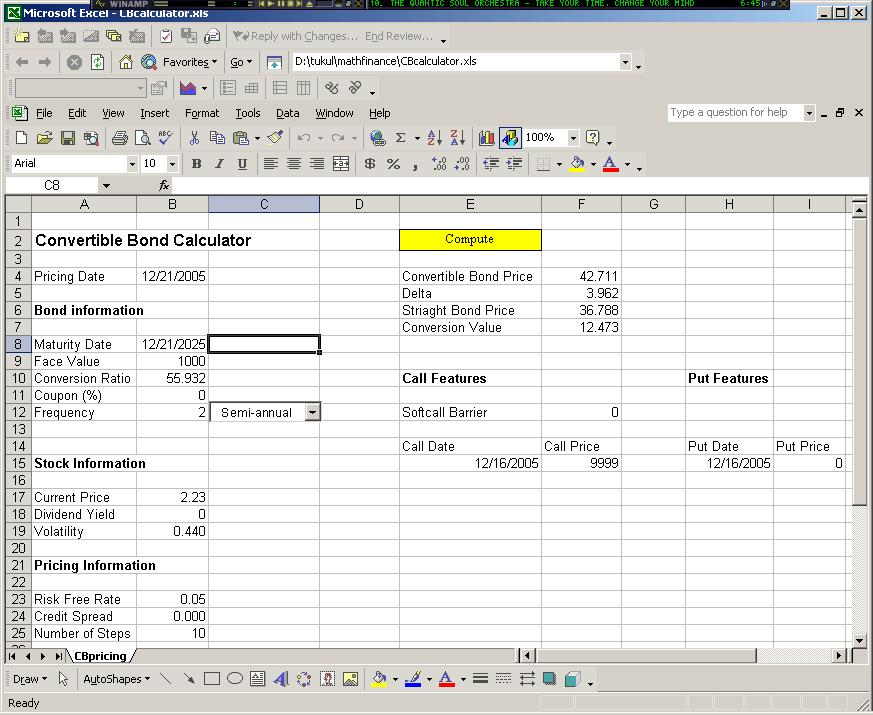
\includegraphics[width=12cm]{cbexample.jpg}
        \caption{Results of pricing of a convertible bond with VBA}
\end{center}
\end{figure}
\begin{figure}
\begin{center}
        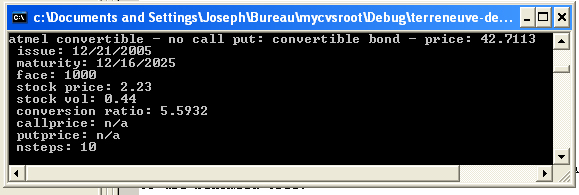
\includegraphics[width=12cm]{cbexample2.jpg}
        \caption{Results of pricing of a convertible bond with our project}
\end{center}
\end{figure}

%\subsection{Pitfalls}

%<i.e. what bugs were found>
